\documentclass{VUMIFPSbakalaurinis}
\usepackage{algorithmicx}
\usepackage{algorithm}
\usepackage{algpseudocode}
\usepackage{amsfonts}
\usepackage{amsmath}
\usepackage{bm}
\usepackage{caption}
\usepackage{color}
\usepackage{float}
\usepackage{graphicx}
\usepackage{listings}
\usepackage{subfig}
\usepackage{wrapfig}

\usepackage{enumitem}
\setitemize{noitemsep,topsep=0pt,parsep=0pt,partopsep=0pt}
\setenumerate{noitemsep,topsep=0pt,parsep=0pt,partopsep=0pt}

% Ignore all trivial warnings
\hbadness=5000
% Titulinio aprašas
\university{Vilniaus universitetas}
\faculty{Informatikos institutas}
\department{Programų sistemų katedra}
\papertype{Bakalauro baigiamasis darbas }
\title{Srautinio apdorojimo modulių generavimas kintant rodiklių duomenų struktūrai}
\titleineng{Generation of Stream Processing Modules upon Change of Indicator Data Structure}
\author{Vytautas Žilinas}
\supervisor{lekt. Andrius Adamonis}
\reviewer{assoc. prof., dr. Karolis Petrauskas}
\date{Vilnius – \the\year}

% Nustatymai
% \setmainfont{Palemonas}   % Pakeisti teksto šriftą į Palemonas (turi būti įdiegtas sistemoje)
\bibliography{bibliografija}

\begin{document} 
\maketitle

\cleardoublepage\pagenumbering{arabic}
\setcounter{page}{2}

\sectionnonumnocontent{Santrauka}
Glaustai aprašomas darbo turinys: pristatoma nagrinėta problema ir padarytos
išvados. Santraukos apimtis ne didesnė nei 0,5 puslapio. Santraukų gale
nurodomi darbo raktiniai žodžiai. 
% Nurodomi iki 5 svarbiausių temos raktinių žodžių (terminų).
% Vienas terminas gali susidėti iš kelių žodžių.
\raktiniaizodziai{raktinis žodis 1, raktinis žodis 2, raktinis žodis 3, raktinis žodis 4, raktinis žodis 5}   

\sectionnonumnocontent{Summary}
Santrauka anglų kalba. Santraukos apimtis ne didesnė nei 0,5 puslapio.
\keywords{keyword 1, keyword 2, keyword 3, keyword 4, keyword 5}

\tableofcontents

\sectionnonum{Įvadas}
 
% TODO: Įžangoje apžvelgti srautinį apdorojimą ir kodo generavimą.
Srautinis duomenų apdorojimas (angl. stream processing) – programavimo paradigma, kuri yra ekvivalenti duomenų srauto programavimo (angl. dataflow programming) paradigmai \cite{shortstreamproc}. 
Duomenų tėkmės programavimo paradigmos idėja yra, kad visa programa susidaro iš skirtingu modulių, kurie nepriklauso vienas nuo kito, ir būtent tai leidžia sukonstruoti paraleliai skaičiuojančias programas. 
Vienas iš pirmųjų duomenų tėkmės programavimo kompiliatorių yra BLODI - blokų diagramų kompiliatorius (angl. BLOck DIagram compiler), su kuriuo buvo kompiliuojamos 
BLODI programavimo kalba parašytos programos \cite{kelly1961block}.  Šia kalba parašytos programos atitinka inžinerinę elektros grandinės schemą, 
kur duomenys keliauja per komponentus kaip ir elektros grandinėje. BLODI kalbos autoriai teigia, kad vienas iš šios programavimo kalbos privalumų yra tas, 
kad ją galėjo išmokti žmonės, kurie nebuvo programavimo ekspertai.\par
Kodo generavimas - todo \par
Šiame darbe nagrinėjamas rodiklių duomenų apdorojimas. Rodiklių duomenimis vadiname duomenis, aprašančius kažkokių objektų savybes arba veiklos procesų rezultatus, 
duomenis galima transformuoti, analizuoti ir grupuoti pagal pasirinktus rodiklius, 
pavyzdžiui: bazinė mėnesinė alga, mirusiųjų skaičius pagal mirties priežastis, krituliai per metus. Taip pat rodiklių struktūra gali keistis laikui bėgant: 
objektų atributų taksonomija (pvz. mirties priežasčių sąrašas, finansinių sąskaitų sąrašas) arba įrašo atributų sąrašai.
Rodiklių duomenų bazės pasižymi tuo, kad duomenys į jas patenka iš daug skirtingų tiekėjų ir patekimo laikas tarp tiekėjų nėra 
sinchronizuojamas, o suagreguotą informaciją vartotojai gali užklausti bet kurio metu.  \par
Vienas iš būdų apdoroti didelius kiekius duomenų gyvai (angl. Real-time data processing) yra srautinis duomenų apdorojimas \cite{BigData, StreamProcessingInData}. 
Dabartinės srautinio apdorojimo sistemos leidžia kurti modulius, kurie apdoroja duomenis ir talpina juos į atskirą talpyklą \cite{8Requirements}. 
Šiame darbe kuriamas sprendimas yra aktualus, kai kinta duomenų struktūra ir norėtume šis sprendimas prisitaiko 
prie duomenų pokyčių kurdamas naujus apdorojimo modulius.

Tikslas: Sukurti rodiklių duomenų srautinio apdorojimo platformos architektūrą, kuri, naudojant kodo generavimą, dinamiškai prisitaiko prie rodiklių duomenų struktūrų pokyčių.

Uždaviniai:
\begin{enumerate}
    \item Apibrėžti rodiklių duomenų modelį ir galimus rodiklių duomenų struktūros pokyčius.
    \item Apibrėžti, kaip specifikuoti duomenų struktūrą ir duomenų struktūrų versijų specifikacijų apjungimo ir skirtumo operacijas.
    \item Atlikus šaltinių analizę pasirinkti srautinio duomenų apdorojimo sistemą, joje sukurti sudarytos architektūros sprendimą ir atlikti bandymus.
\end{enumerate}

\section{Rodiklių duomenys}

Rodiklių duomenys - tai duomenis, kurie apibrėžia bet kokius gyvenimiškus duomenis, kuriuos galime grupuoti pagal tam tikrus raktinius elementus. Rodiklį sudaro pirminis raktas arba raktų rinkinys ir reikšmių sąrašas, kurį galime grupuoti pagal apibrėžtus raktus.      

\subsection{Rodiklių duomenų modelis}

Darbo tikslui išpildyti buvo sukurtas modelis, kurio pagalba galime apibrėžti rodiklį. Pagal šį apibrėžimą bus generuojama srautinio apdorojimo architektūra.

\begin{figure}[H]
    \centering
    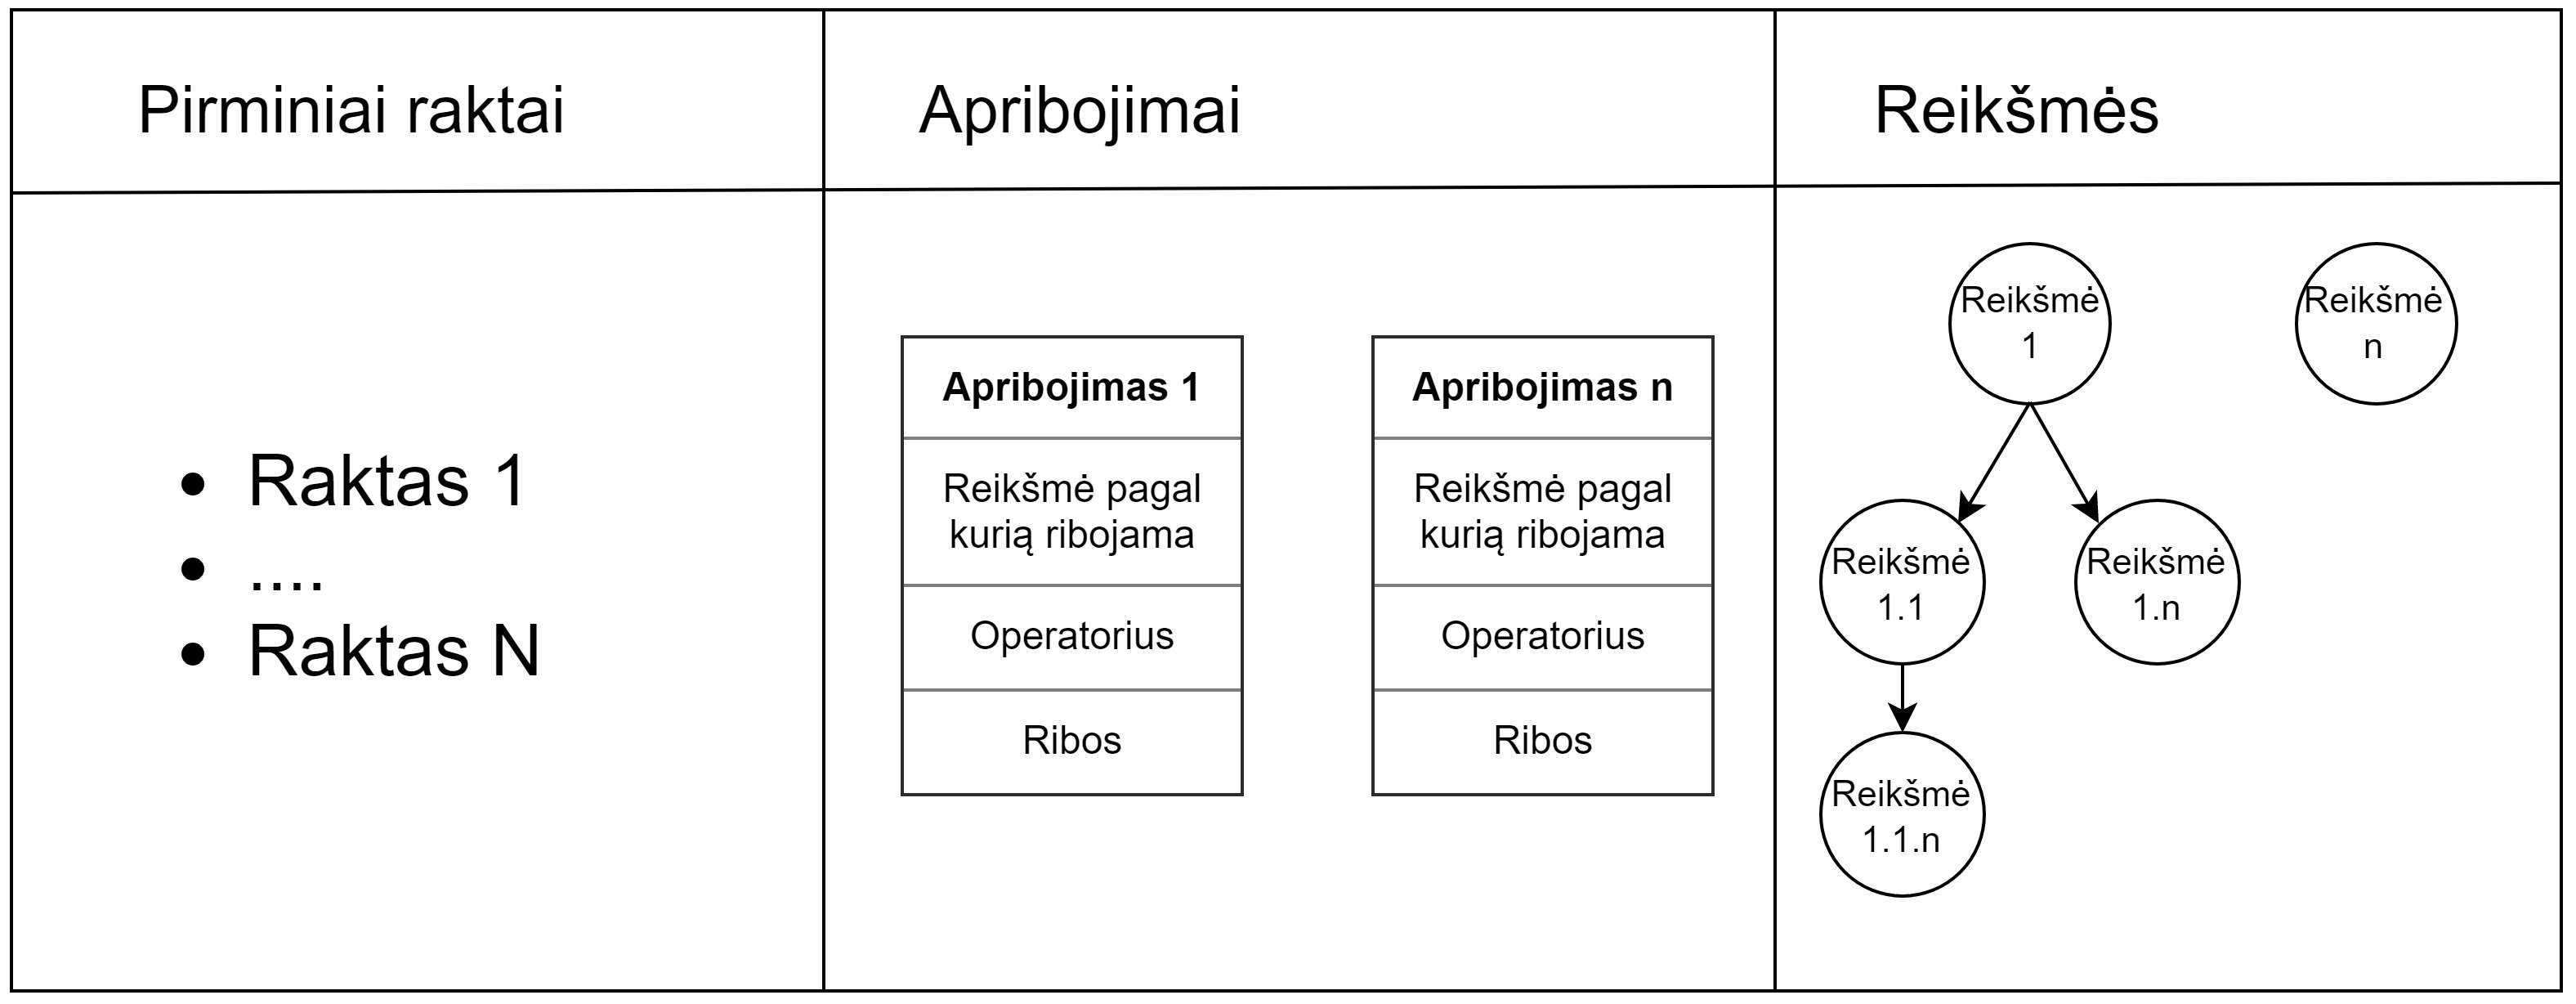
\includegraphics[width=1\textwidth]{img/Rodiklis}
    \caption{Rodiklis}
    \label{img:rodiklis}
\end{figure}


\subsection{Rodiklių duomenų struktūros pokyčiai}

\section{Medžiagos darbo tema dėstymo skyriai}
Medžiagos darbo tema dėstymo skyriuose išsamiai pateikiamos nagrinėjamos temos
detalės: pradiniai duomenys, jų analizės ir apdorojimo metodai, sprendimų
įgyvendinimas, gautų rezultatų apibendrinimas.

Medžiaga turi būti dėstoma aiškiai, pateikiant argumentus. Tekste dėstomas
trečiuoju asmeniu, t.y. rašoma ne „aš manau“, bet „autorius mano“, „autoriaus
nuomone“. Reikėtų vengti informacijos nesuteikiančių frazių, pvz., „...kaip jau
buvo minėta...“, „...kaip visiems žinoma...“ ir pan., vengti grožinės
literatūros ar publicistinio stiliaus, gausių metaforų ar panašių meninės
išraiškos priemonių.

Skyriai gali turėti poskyrius ir smulkesnes sudėtines dalis, kaip punktus ir
papunkčius.

\sectionnonum{Rezultatai}

\begin{enumerate}
    \item Apibrėžta rodiklių duomenų struktūra ir galimi duomenų struktūros pokyčiai.
    \item Pasirinktai srautinio duomenų apdorojimo sistemai sukurto sprendimo atliktų eksperimentų rezultatai - generuojamas kodas ir jo savybes. 
\end{enumerate}

\sectionnonum{Išvados}
Rezultatų ir išvadų dalyje išdėstomi pagrindiniai darbo rezultatai (kažkas
išanalizuota, kažkas sukurta, kažkas įdiegta), toliau pateikiamos išvados
(daromi nagrinėtų problemų sprendimo metodų palyginimai, siūlomos
rekomendacijos, akcentuojamos naujovės). Rezultatai ir išvados pateikiami
sunumeruotų (gali būti hierarchiniai) sąrašų pavidalu. Darbo rezultatai turi
atitikti darbo tikslą.

\printbibliography[heading=bibintoc] 


\appendix 


\end{document}
